\chapter{Locality and Caches}
\label{chap:locality}

For modern computers, computation is a rather cheap operation in terms
of time and energy consumption.  In fact, it is far more
energy-consuming and slow to \emph{move} data than to perform
computation.  As we discussed in \cref{chap:bytes}, program data is
usually stored in memory and must be moved into CPU registers before
it can be worked on.  Particularly large quantities of data might not
even fit in memory, but is stored in local or remote files.  The
details can differ, but in all cases the situation is the same: data
must be moved from \emph{over there} to \emph{here} before it can be
used.

This phenomenon that computation is faster than memory, is often
called the \emph{memory wall}, and the gap is still widening.  While
faster processors keep getting designed, memory technology is not
keeping up, and therefore we have increasing difficulty supplying our
processors with data.

Since data movement is slow and costly compared to computation, a
programmer who wants to write high-performance code must be diligent
in doing as little of it as possible.  This chapter describes the
properties of software and hardware that one must exploit to
accomplish this.

While we will continue to use C for concrete programming examples, the
principles here are truly universal, and inescapable whenever we write
code for modern computers.  Fortunately, we will see that optimising
code to minimise data movement usually doesn't require us to write
particularly ugly or complicated code - it is mostly about choosing
the right data structures and traversing them in a sensible manner.

\section{Locality of Reference}

Empirically, programs tend to access data located nearby data that was
accessed recently.  We call this phenomenon the \emph{principle of
  localty}.

\begin{definition}[Principle of locality]
  Programs tend to access data located near that which was accessed
  recently.
\end{definition}

To keep things simple, this chapters is concerned only with data
stored in memory, and we will decide if two pieces of data are
``close'' to each other based on the numerical value of their
addresses.  For example, the byte at address $100$ is considered
adjacent to the bytes at addresses $99$ and $101$.  However, some
notion of locality is present in any kind of storage technology.
Informally, we say that a program ``exhibits good locality'' when it
adheres to the principle of locality.

The principle of locality is what ultimately helps us break through
the memory wall.  It is a virtuous cycle: we build computers that take
run programs with good locality more quickly, which makes programs try
to improve the locality in their programs.

We distinguish between two kinds of locality.

\begin{definition}[Temporal locality]
  Accessing data that was accessed recently.
\end{definition}

\begin{definition}[Spatial locality]
  Accesing data close to data that was accessed recently.
\end{definition}

While it is possible to run a program, record the exact memory
operations performed, and then quantiatively describe how much
locality they exhibit, this is often somewhat impractical.  Instead, a
good programmer should develop the ability to quickly eyeball simple
programs and qualitiatively estimate their locality.

\subsection{Qualitative Estimates of Locality}

\begin{figure}
\begin{lstlisting}[
caption={C code that sums an array.},
label={lst:locality-example},
language=C,
frame=single]
double sum = 0;
for (int i = 0; i < n; i++) {
  sum += a[i];
}
\end{lstlisting}
\end{figure}

Consider the program fragment shown in \cref{lst:locality-example}.
In terms of data accesses, it accesses the elements of the array
\texttt{a} serially, with a \emph{stride} of $1$ between successive
accesses.  This is an example of \emph{spatial locality}: we do not
access the same data, but we do access data very close to what we
accessed in the recent past.  Further, we also repeatedly access the
variables \texttt{sum} and \texttt{i}. This is an example of
\emph{temporal locality}.

But program data is not the only thing that is stored in memory: the
program \emph{code} is as well, in the form of machine instructions.
Absent of control flow, instructions are read from memory and executed
in the order in which they appear---just like how lines in a C program
are executed from the top down.  This means they have \emph{spatial
  locality}.  However, we also have a loop in
\cref{lst:locality-example}, which means that the same instructions
are executed repeatedly.  This is \emph{temporal locality}.  Generally
speaking, program code almost always exhibits good locality, so we
tend to ignore it when analysing the locality of a program, and
instead focus only on the locality of data accesses.

Further, we focus only on memory accesses.  Because simple scalar
variables tend to be stored in registers by the C compiler, we look
only at how arrays are traversed.

\subsection{Analysing Array Iteration}

\begin{figure}
\begin{lstlisting}[
caption={Summing a matrix, iterating along the rows.},
label={lst:locality-sumrows},
language=C,
frame=single]
int sumrows(int A[M][N]) {
  int sum = 0;
  for (int i = 0; i < M; i++)
    for (int j = 0; j < N; j++)
      sum += A[i][j];
  return sum;
}
\end{lstlisting}
\end{figure}

Let us consider a more complicated example, seen in
\cref{lst:locality-sumrows}.  For concision we are use
multidimensional C arrays, rather than explicit index functions as in
\cref{chap:datalayout}.  This means that the array \texttt{A} is
stored in row-major order and that the access \texttt{A[i][j]} results
in an offset computation \texttt{i*N+j}.

Consider the memory accesses performed by the loop.  In the first
iteration, we have \texttt{i=0} and \texttt{j=0}, meaning that we
access memory at offset \texttt{0}.  In the next iteration we have
\texttt{i=0} and \texttt{j=1}, meaning we access offset
\texttt{1}\footnote{Strictly speaking, we are accessing
  \texttt{1*sizeof(int)}, meaning \texttt{4}, but since the first
  iteration accesses the four bytes stored at offsets \texttt{0-3},
  this is still considered adjacent.  We can ignore the element size
  for arrays of scalars, but it does have impact if we have arrays
  containing large compound data structures.}.  In every loop
iteration, we will access an array element adjacent to the one
accessed in the immediately preceding iteration---the stride is
$1$---and therefore this function exhibits good spatial locality with
respect to how it accesses \texttt{A}.

\begin{figure}
\begin{lstlisting}[
caption={Summing the rows of a matrix, iterating along the columns},
label={lst:locality-sumcols},
language=C,
frame=single]
int sumcols(int A[M][N]) {
  int sum = 0;
  for (int j = 0; j < N; j++)
    for (int i = 0; i < M; i++)
      sum += A[i][j];
  return sum;
}
\end{lstlisting}
\end{figure}

Now consider \cref{lst:locality-sumcols}.  By repeating the analysis
above, we see that the first array element we access is
\texttt{A[0][0]} and the next one is \texttt{A[1][0]}.  Since
\texttt{A} is stored in row-major order, this means we are iterating
with a stride of \texttt{N}.  Assuming \texttt{N} is large, this
function exhibits \emph{bad} locality with respect to \texttt{A}.

\section{Memory Hierarchies}

In an ideal world, memory would be cheap, fast, and plentiful.  In the
world we actually inhabit, we cannot get all three.  In fact,
fundamental physical principles mean memory capacity and memory
capacity are conflicting properties.  Roughly, the larger the capacity
of some storage technology, the longer it takes it to retrieve data.
However, by exploiting the principle of locality, we can construct a
\emph{memory hierarchy} of different storage technologies, starting
from the small and fast and ending in the large and slow.

\begin{definition}[Memory hierarchy]
  A separation of computer storage into levels based on their response
  time and capacity.
\end{definition}

The idea behind a memory hierarchy is that each level contains a
\emph{subset} of the data contained in the level below it.  Only the
level at the bottom contains \emph{all} data.  Each level of the
hierarchy acts as a \emph{cache} for the one below it.

\begin{definition}[Cache]
  A smaller and faster memory that stores a subset of the contents of
  a larger and slower memory.
\end{definition}


\begin{figure}
  \centering

  \begin{center}
    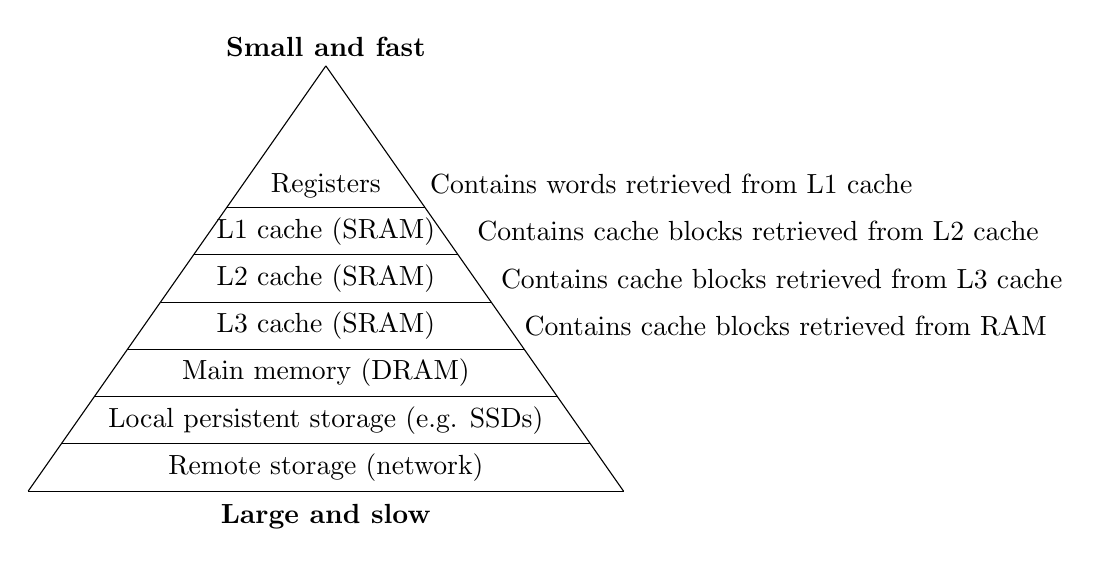
\begin{tikzpicture}[scale=0.6]
      \def \h {9};
      \def \f {.7};

      \foreach \y in  {0,1,2,3,4,5,6} {
        \def \w { \h*\f-\y*\f };
        \def \v { \y*\f-\h*\f };
        \draw (\v,\y) -- (\w,\y);
      }

      \draw (-\h*\f,0)  -- (0,\h);
      \draw (\h*\f,0)  -- (0,\h);

      \node at (0,0) [above] {Remote storage (network)};
      \node at (0,1) [above] {Local persistent storage (e.g. SSDs)};
      \node at (0,2) [above] {Main memory (DRAM)};
      \node at (0,3) [above] {L3 cache (SRAM)};
      \node[align=left] at (4,3.5) [right] {Contains cache blocks retrieved from RAM};
      \node at (0,4) [above] {L2 cache (SRAM)};
      \node[align=left] at (3.5,4.5) [right] {Contains cache blocks retrieved from L3 cache};
      \node at (0,5) [above] {L1 cache (SRAM)};
      \node[align=left] at (3,5.5) [right] {Contains cache blocks retrieved from L2 cache};
      \node at (0,6) [above] {Registers};
      \node at (2,6.5) [right] {Contains words retrieved from L1 cache};

      \node at (0,9) [above] {\textbf{Small and fast}};
      \node at (0,-1) [above] {\textbf{Large and slow}};
    \end{tikzpicture}
  \end{center}

  \caption{Example memory hierarchy for a modern computer.  The number
    of levels and the specifics of their operation depends on the
    computer in question.  Very tiny computers may have no caches at
    all, but only registers and main memory.  Some extremely small
    processors may have only registers---but these are unlikely to be
    useful for general-purpose computation.}
  \label{fig:memory-hierarchy}
\end{figure}

An example of a memory hierarchy for a computer is shown in
\cref{fig:memory-hierarchy}.  The exact levels of the memory hierarchy
depends on the machine.  Further, when using the memory hierarchy
model to describe the performance of a system, we often exclude levels
that are irrelevant---for example, registers are often ignored because
they are controlled by the compiler, and we might ignore anything
below main memory if we know that our data will fit.

In this chapter we will focus entirely how the contents of RAM is
cached.  Further, while real computers usually have multiple levels of
caching, we will for simplicity asumme only a single level above main
memory, and just call it \emph{the cache}.  So in total, we pretend we
have only two levels: the small and fast cache on top, and the large
and slow main memory below it.  In a full memory hierarchy, this
situation is simply replicated for each levelall the way down.

\subsection{Cache Operation}

The reason why caching works is due to the principle of locality: most
accesses will tend to be towards the top of the hierarchy.  When we
try to access an address that is already present in the cache, the
data is immediately returned to the program.

\begin{definition}[Cache hit]
  A memory operation to an address that is present in the cache.
\end{definition}

If we try to retrieve a piece of data that is not already in the
cache, the data is fetched from the next level of the hierarchy,
stored in the cache, and then returned to the program.

\begin{definition}[Cache miss]
  A memory operation to an address that is not present in the cache.
\end{definition}

In programs with good locality, most memory accesses will result in
cache hits.  For such programs, the memory hierarchy provides the
illusion of storage that is as large as the bottommost level of the
hierarchy, and as fast as the topmost one.

If caches merely contained \emph{exactly} the bytes that had been
retrieved previously, then only temporal locality would benefit.
Instead, we partition the addressable memory space into \emph{cache
  blocks}, each containing $B$ bytes.

\begin{definition}[Cache block]
  A $B$-byte chunk of memory, where $B$ is a power of two.
\end{definition}

Whenever we have a cache miss, the entire block containing the
requested address is copied into the cache.  This means that
subsequent accesses to addresses that fall within the same block will
result in cache hits.  This means that programs that exhibit good
spatial locality will have more cache hits.

On modern computers, $B=64$ is common.  It is important to be aware
that the organisation of memory into cache blocks does not affect
addressing: data is still byte-addressed, and programs are not
directly aware of $B$.  We merely say that the first $B$ bytes of
memory belong to the first cache block, the next $B$ bytes to the
second, and so on.  This means a memory address $x$ belongs to block
$x mod B$.  When $B$ is a power of 2 $B=2^{m}$, this can be computed
simply by dropping the $b$ least significant bits of $m$.  We will
return to this in \cref{sec:cache-organisation}.  Each level of the
memory hierarchy may use different cache block sizes, although they
are usually the same for the L1/L2/L3 caches.

Caching is effective when the data being actively actively by the
program within some bounded period of time fits within the cache.  We
call the size of this actively used data the \emph{working set}.

\begin{definition}[Working set]
  The amount of memory accessed by a program within a bounded period
  of time.
\end{definition}

\begin{definition}[Memory footprint]
  The total amount of memory allocated by a program.
\end{definition}

During the total runtime of a process, different working sets may be
in use, as the program switches between different subtasks.  Consider
a data analysis program sequentially processes a collection of files,
one at a time, by loading them into memory.  We would characterise the
working set of such a program as the size of a \emph{single} file
(perhaps the largest one), rather than summing the sizes of all files.
We also focus only on data that is being frequently accessed.  It is
fine for the total memory footprint of a program to exceed what can be
stored in the cache, as the excess is simply stored further down in
the memory hierarchy.  It is not unusual for programs to keep large
amounts of data in memory at the same time, while actively working on
only small parts at a time.  Indeed, this is exactly how to make best
use of the memory hierarchy.

\begin{definition}[Compulsory miss]
  A miss that occurs because the cache is empty.
\end{definition}

\begin{definition}[Conflict miss]
  A miss that occurs because too many blocks of the program working
  set are mapped to the same cache set.
\end{definition}

\begin{definition}[Capacity miss]
  A miss that occurs because the program working set exceeds the cache
  capacity.
\end{definition}

\section{Cache Organisation}
\label{sec:cache-organisation}

\begin{definition}[Cache line]
  A structure that contains a cache block as well as metadata about
  the origin of the block.
\end{definition}

When $S=2^{n}, B=2^{m}$ we can easily split a $w$-bit address into
\emph{fields}, writing $x_{i}$ for bit $i$.

  \[
    \underbrace{x_{w-1}\cdots{}x_{m+n+1}}_{\text{tag}}
    \underbrace{x_{m+n}\cdots{}x_{m}}_{\text{set index}}
    \underbrace{x_{m-1}\cdots{}x_{0}}_{\text{block offset}}
  \]

  \begin{example}[Fields for an 8-bit address scheme]
    Consider an $8$-bit address on a system with a block size of
    $2^{m}$ and $2^{s}$ sets, with $m=2,s=3$.  Going from right to
    left, the first $m$ bits constitute the offset, the next $s$ bits
    the set index, and the remainder are the tag.
    \[
      \underbrace{x_{7}x_{6}x_{5}}_{\text{tag}}
      \underbrace{x_{4}x_{3}x_{2}}_{\text{tag}}
      \underbrace{x_{1}x_{0}}_{\text{offset}}
    \]
  \end{example}

\section{Cache Performance}

%%% Local Variables:
%%% mode: latex
%%% TeX-master: "notes"
%%% End:
